\section{Overview}
\label{ch1:sec:overview}

The algorithm contains two parts:  a training scenario and a production scenario.
Both implement Reinforcement Learning and have a co-simulation engine. 
However, the first one co-simulates with OpenDSS via COM interface and does not have 
prior knowledge about the distribution network; while, the second one co-simulates 
with OpenDSS-G through TCP/IP protocol and does know the distribution network dynamics. 
The co-simulation engine differs from scenarios due to performance.
OpenDSS-G adds a graphic user interface which helps to visualize the topology of the 
distribution network and its changes, but also adds more processing time compared with OpenDSS. 

The SR algorithm is written in Python 3.7 and has an Objet Oriented Programming structure.
Also, it requires the following input data from the distribution network: lines, switches, 
the state of the switches, bus voltages, line currents, load powers, and incidence matrix. 

According to this, Figure \ref{ch1:fig:rl_scenarios} presents the general SR algorithm block diagram.

\begin{figure}
    \centering
    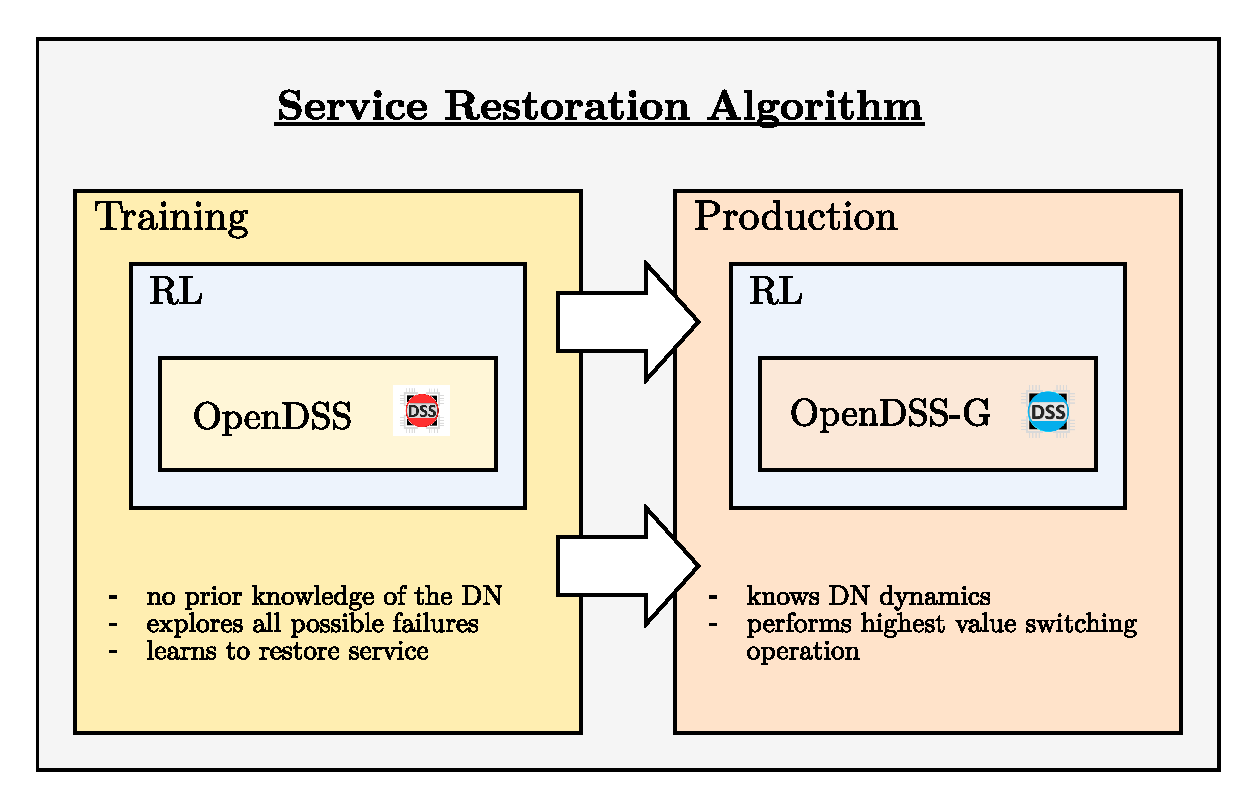
\includegraphics[scale=0.6]{_chapter1/fig/rl_scenarios.pdf}
    \caption{RL scenarios}
    \label{ch1:fig:rl_scenarios}
\end{figure}